\section{Datasets}\label{sec:datasets}
\subsection{Data and Triggers}

This analysis uses certified events from the Run 2016B-H datasets corresponding to $35.9~\text{fb}^{-1}$. 
It uses control regions defined by muons, and electrons, so the MET and SingleElectron primary datasets are used. 
The MET dataset includes muon pass-through triggers, which allow us to select events with high $\MET$ or high muon recoil. 
A list of all triggers is given in Table~\ref{tab:trigs}. 

\begin{table}[h]
\scriptsize
    \centering
    \begin{tabular}{l|c|c}
\hline
\hline %--------------------------------------------------------------------------------------------------------------------------                
HLT path                                         & L1 seed                   & Primary dataset \\
\hline %--------------------------------------------------------------------------------------------------------------------------                
\verb| HLT_PFMET170_*                          | & \begin{tabular}{c@{}c@{}} \verb| L1_ETM70 or L1_ETM100      | \end{tabular}                                                     & MET \\
\hline
\verb| HLT_PFMETNoMu[X]_PFMHTNoMu[X]_IDTight   | & \begin{tabular}{c@{}c@{}} \verb| L1_ETM70 or L1_ETM100      | \\ \verb| L1_ETM60_NotJet52WdPhi2 | \end{tabular}                 & MET \\
\hline
\hline
\verb| HLT_Ele27_WPTight                       | & \begin{tabular}{c@{}c@{}} \verb| L1_SingleEG20 | \\ \verb| L1_SingleIsoEG18er      | \\ \verb| L1_SingleIsoEG20 | \end{tabular} & SingleElectron \\
\hline
\verb| HLT_Ele105_CaloIdVT_GsfTrkIdT           | & \begin{tabular}{c@{}c@{}} \verb| L1_SingleEG40 | \\ \verb| L1_SingleJet200         | \end{tabular}                              & SingleElectron \\
\hline
\hline %--------------------------------------------------------------------------------------------------------------------------              
    \end{tabular}
\small
   \caption{HLT paths, and the associated L1 seeds used in the analysis. In the case of the $NoMu$ triggers, the lowest un-prescaled triggers at different stages of data-taking have a different threshold on PFMETNoMu and PFMHTNoMu. Therefore `[X]' in the trigger path name stands for 90 or 100 or 110 or 120\,GeV.}
   \label{tab:trigs}
\end{table}


The offline cuts are chosen such that the triggers are near 100\% efficiency. 
Triggers are applied to data events.
To simulate the effect of MET and SingleElectron triggers on data, efficiency factors are applied to Monte Carlo events.
The measurement of these efficiencies is further described in Ref~\cite{CMS_AN_2016-473}.
%The trigger efficiencies are functions of muon recoil (for MET), and electron $p_T,\eta$ (SingleElectron). 
The efficiencies for all the triggers are shown in Figures~\ref{fig:hlteff_met}-\ref{fig:eltrigsfsplot}.

As shown in Figure~\ref{fig:triggerComparison_wmn_zmm}, it has been noticed by comparing the trigger efficiency measured in \Zmm~selection and \Wmn~selection (starting from events recorder by single-muon triggers) that these two measurements differed which implies that application of the efficiency curve derived in the \Wmn~control region to \Zmm~events might not be correct. The difference has been observed both on data and MC. The absence of prescale information in MC causes a difference in the turn on position respect to what is measured on data, where only PFMetNoMu120 was fully unprescaled along the data taking. Eventually, simulated \Zmm~events are corrected in the analysis using the proper trigger efficiency as derived from \Zmm~candidates in data and the full difference between the \Wmn~and the \Zmm~trigger turn on is used as systematic uncertainty due to the \MET triggers and applied to the transfer factors as described in Section~\ref{systematics}. The weights after the correction and the assigned uncertainties are presented in Figures~\ref{fig:trigger_eff_corr}-\ref{fig:fixtrig_monoh}.

%\subsection{Photon Trigger Performance}\label{sec:gamtriggerperformance}
%The single photon triggers are employed to select events that are used in the \phojets~control region.
%We take a logical OR of three single photon triggers.
%The performance of the trigger is measured in events passing the PFHT650. These events are required to have a single photon in the barrel
%($|\eta| < 1.4442$) passing the tight selection employed in the analysis. %The efficiency of the single photon triggers is shown as a function of photon \pt in Fig.\ref{fig:hlteff_pho} using blue points. We see that the trigger efficiency is around 0.98 for a photon \pt up to 500 GeV and then starts dropping. This inefficiency is due to a misconfiguration of the EGamma L1 seed. This efficiency loss can be largely recovered by taking a logical OR of the single photon triggers with the lowest unprescaled HT trigger, namely the PFHT800 trigger. The red points in Fig.\ref{fig:hlteff_pho} show the trigger efficiency after adding the PFHT800 trigger. There is still some loss in efficiency (2-3\%) for photon \pt between 200 to 400 GeV, but beyond that range the efficiency rises quickly to unity. Same measurement is also peformed with respect to a single jet trigger (HLT\_PFJet320) in the JETHT dataset with and without recovery. Fig.~\ref{fig:hlteff_pho_singlejet} shows the trigger efficiency before/after adding the recovery triggers.


%\subsection{Electron Trigger Performance}\label{sec:eletriggerperformance}
For the single and double electron control regions we select events that pass a logical OR of different Ele27 and Ele105 triggers. Depending on the $p_\text{T}$ threshold of the electron triggers, they employ different criteria on the identification and isolation. 
%The Ele27 trigger has tight identification and isolation requirements whereas the Ele105 trigger has loose identification and no isolation requirements. 
The Ele27 trigger suffers from some inefficiency for $Z\to ee$ events in which the Z boson is boosted. In such events the two electrons can spoil each others isolation at the trigger. Therefore, adding the Ele105 trigger which has no isolation requirement helps to recover this inefficiency.

The efficiency of the electron triggers used is measured in data using two approaches. We use the tag-and-probe technique in which the trigger efficiency is measured on an electron leg of the Z boson. Events are selected requiring one tag electron which fires the single electron triggers and passes the tight identification requirements. Then a second probe electron is also required in the event. The probe electron is also required to pass the tight selection, and the invariant mass of the dielectron pair is required to be consistent with the Z peak. Then the fraction of events in which the probe electron fires the trigger gives the trigger efficiency. The trigger efficiency is measured in bins of the \pt and $\eta$ of the electron. The drawback of the tag-and-probe approach is that we run out of Z events at high electron \pt. Therefore, to complement this measurement we measure the electron efficiency in events from the JetHT passing the PFHT800 trigger. %This procedure is similar to the efficiency measurement of the photon triggers. %Fig.~\ref{fig:trigs} shows the trigger efficiency measured in bins of electron \pt and $\eta$. 
In the case of electrons with \pt less than 100 \GeV, the trigger efficiency is taken from the Z tag-n-probe measurement. In the case of electrons with \pt greater than 100 \GeV, the trigger efficiency is taken from the JetHT data.



%\begin{figure}[htbp]
%   \centering
%         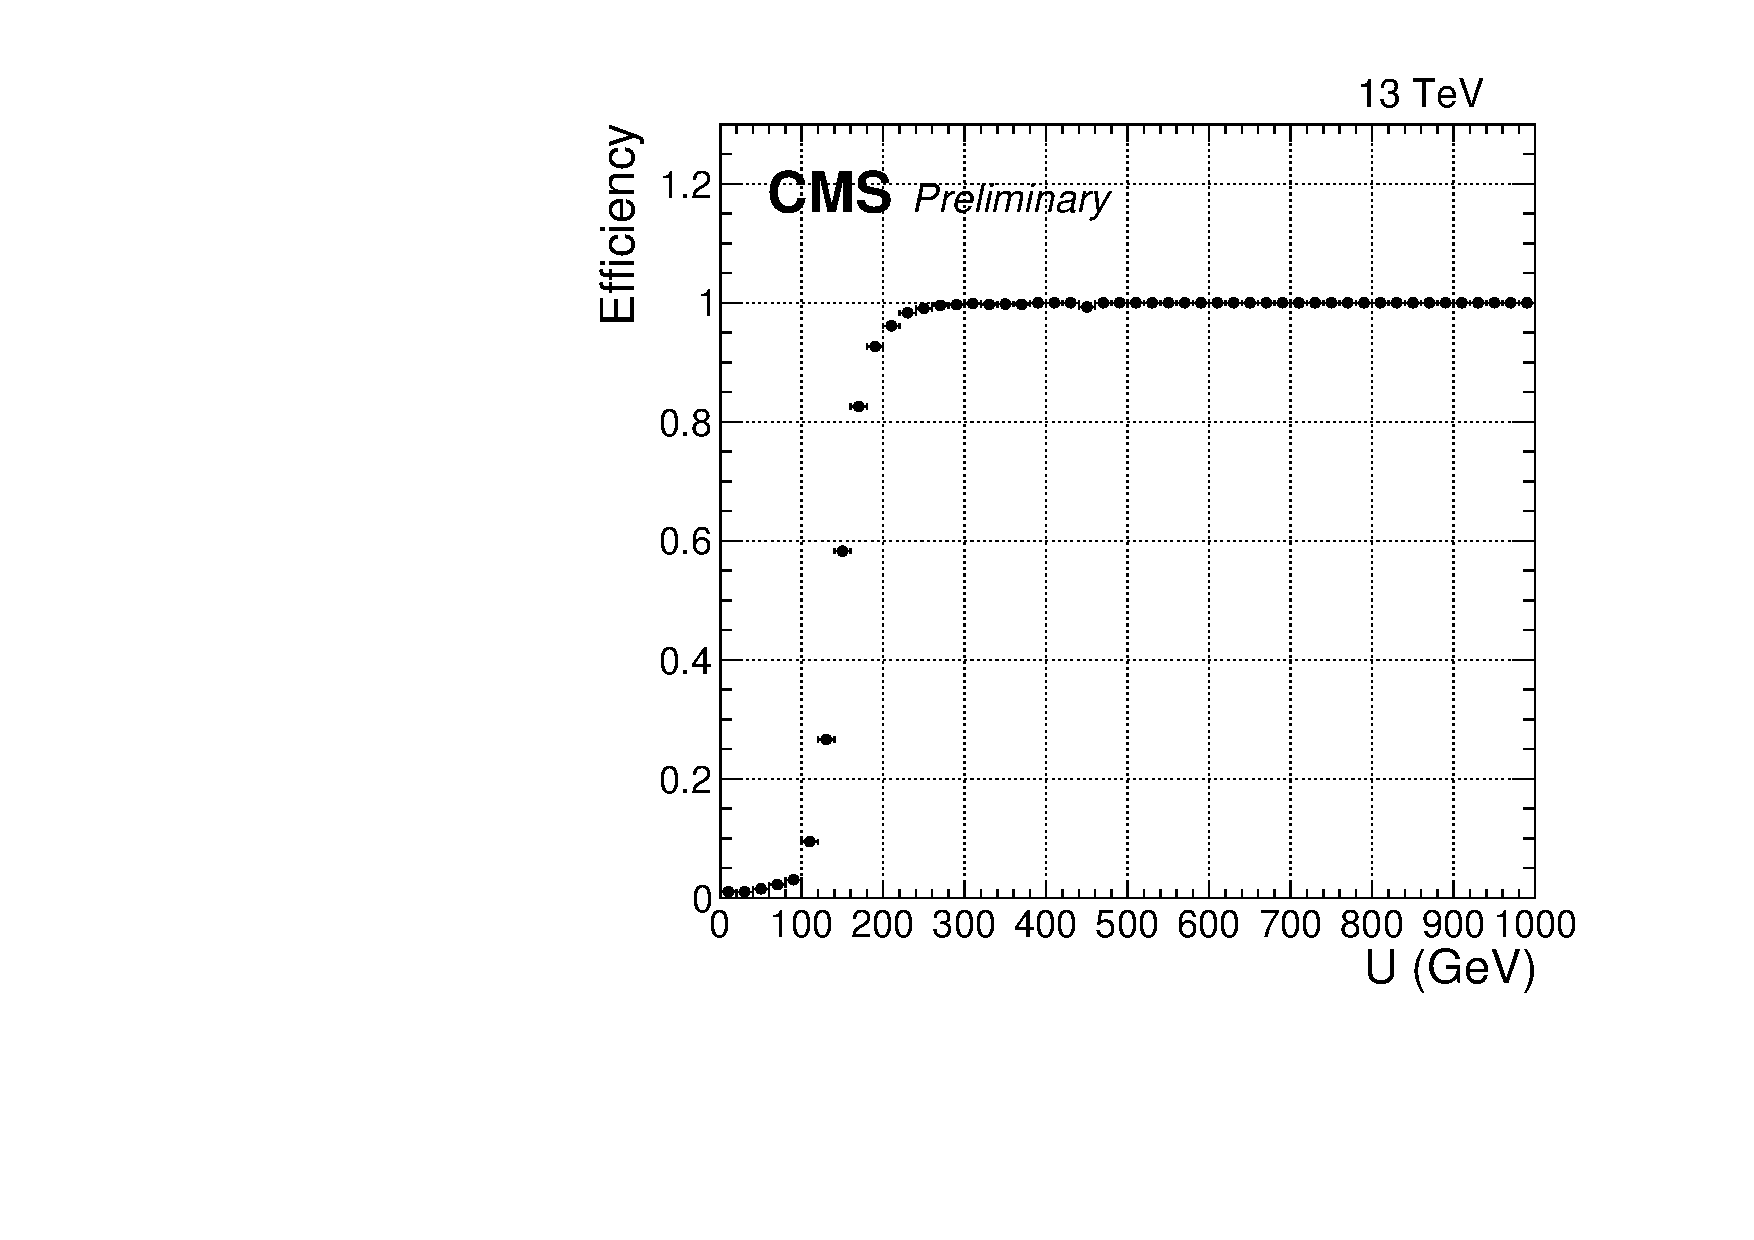
\includegraphics[width=0.475\textwidth]{figures/trigs/met_trig.pdf}
%         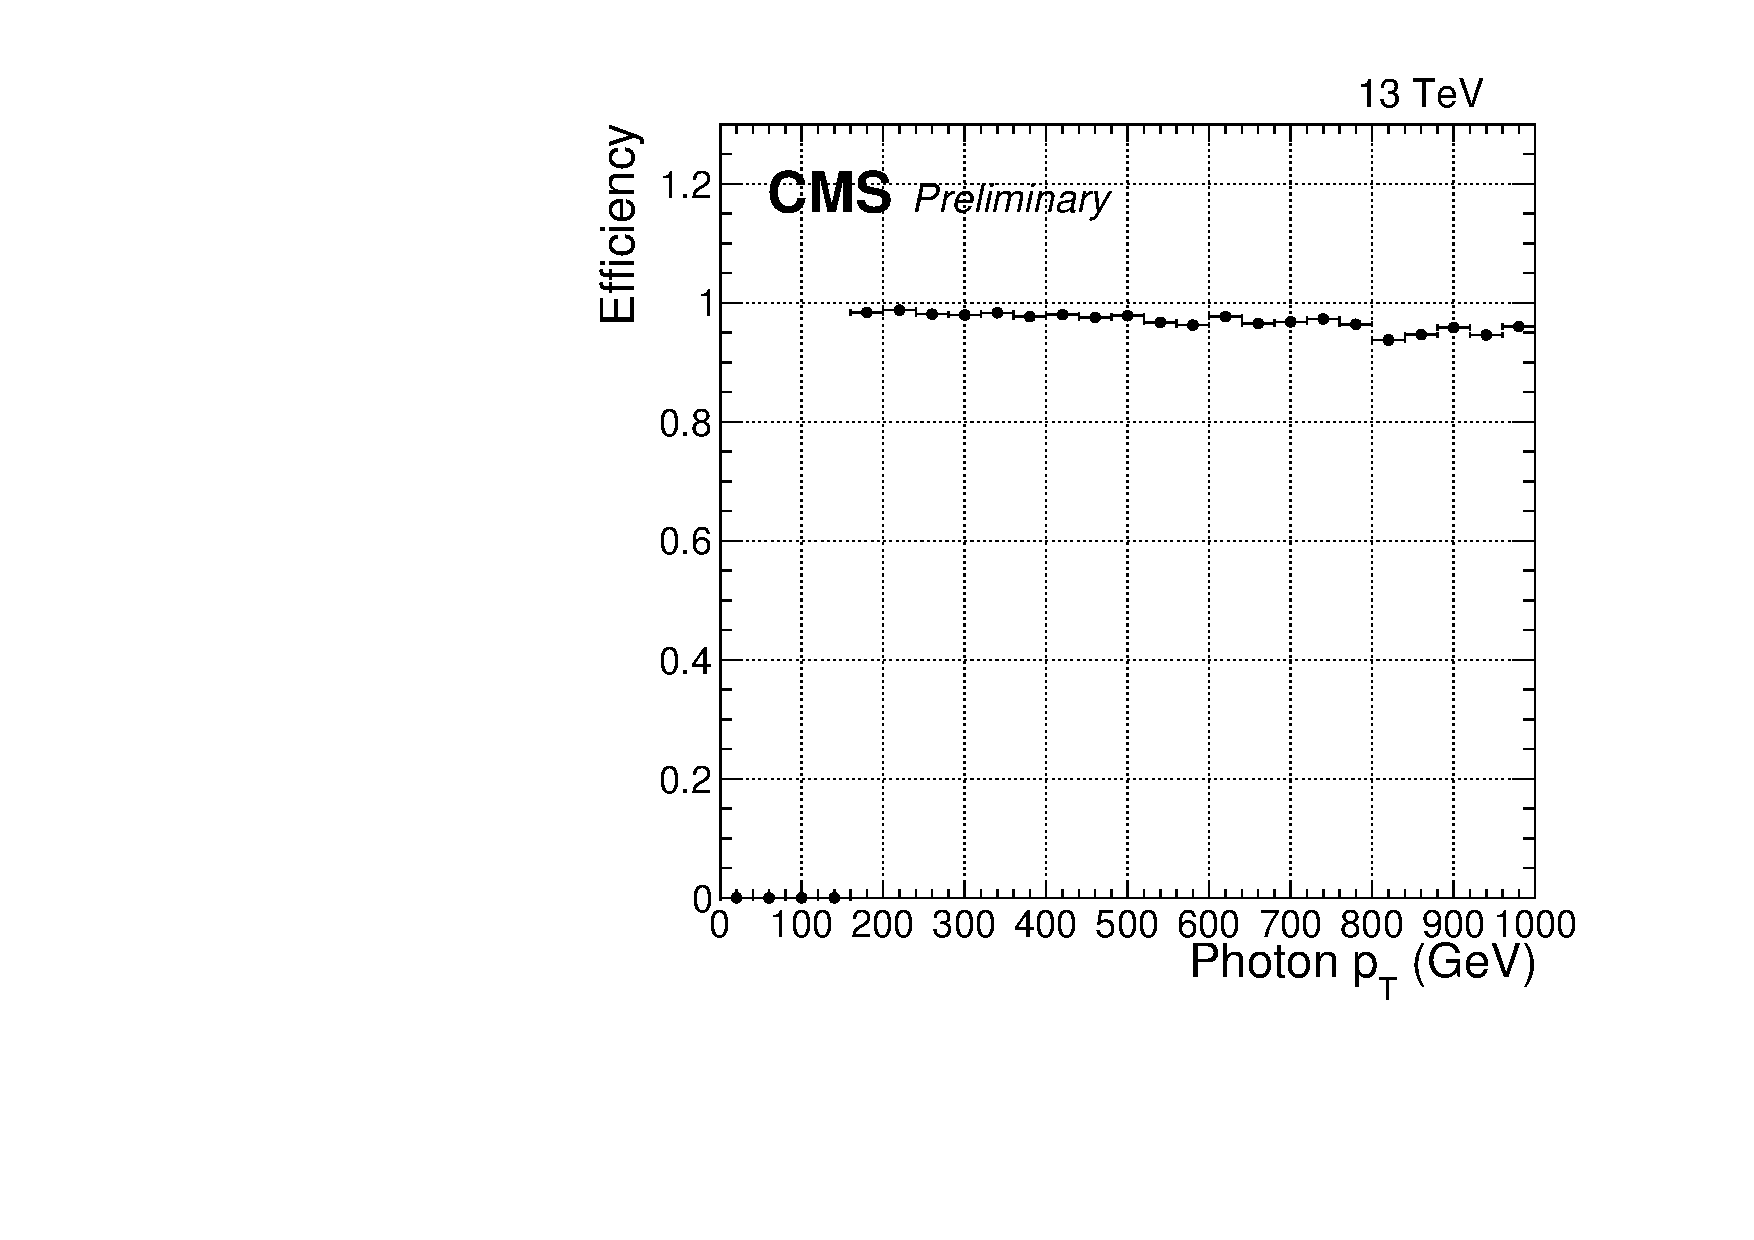
\includegraphics[width=0.475\textwidth]{figures/trigs/photon_trig.pdf}\\
%         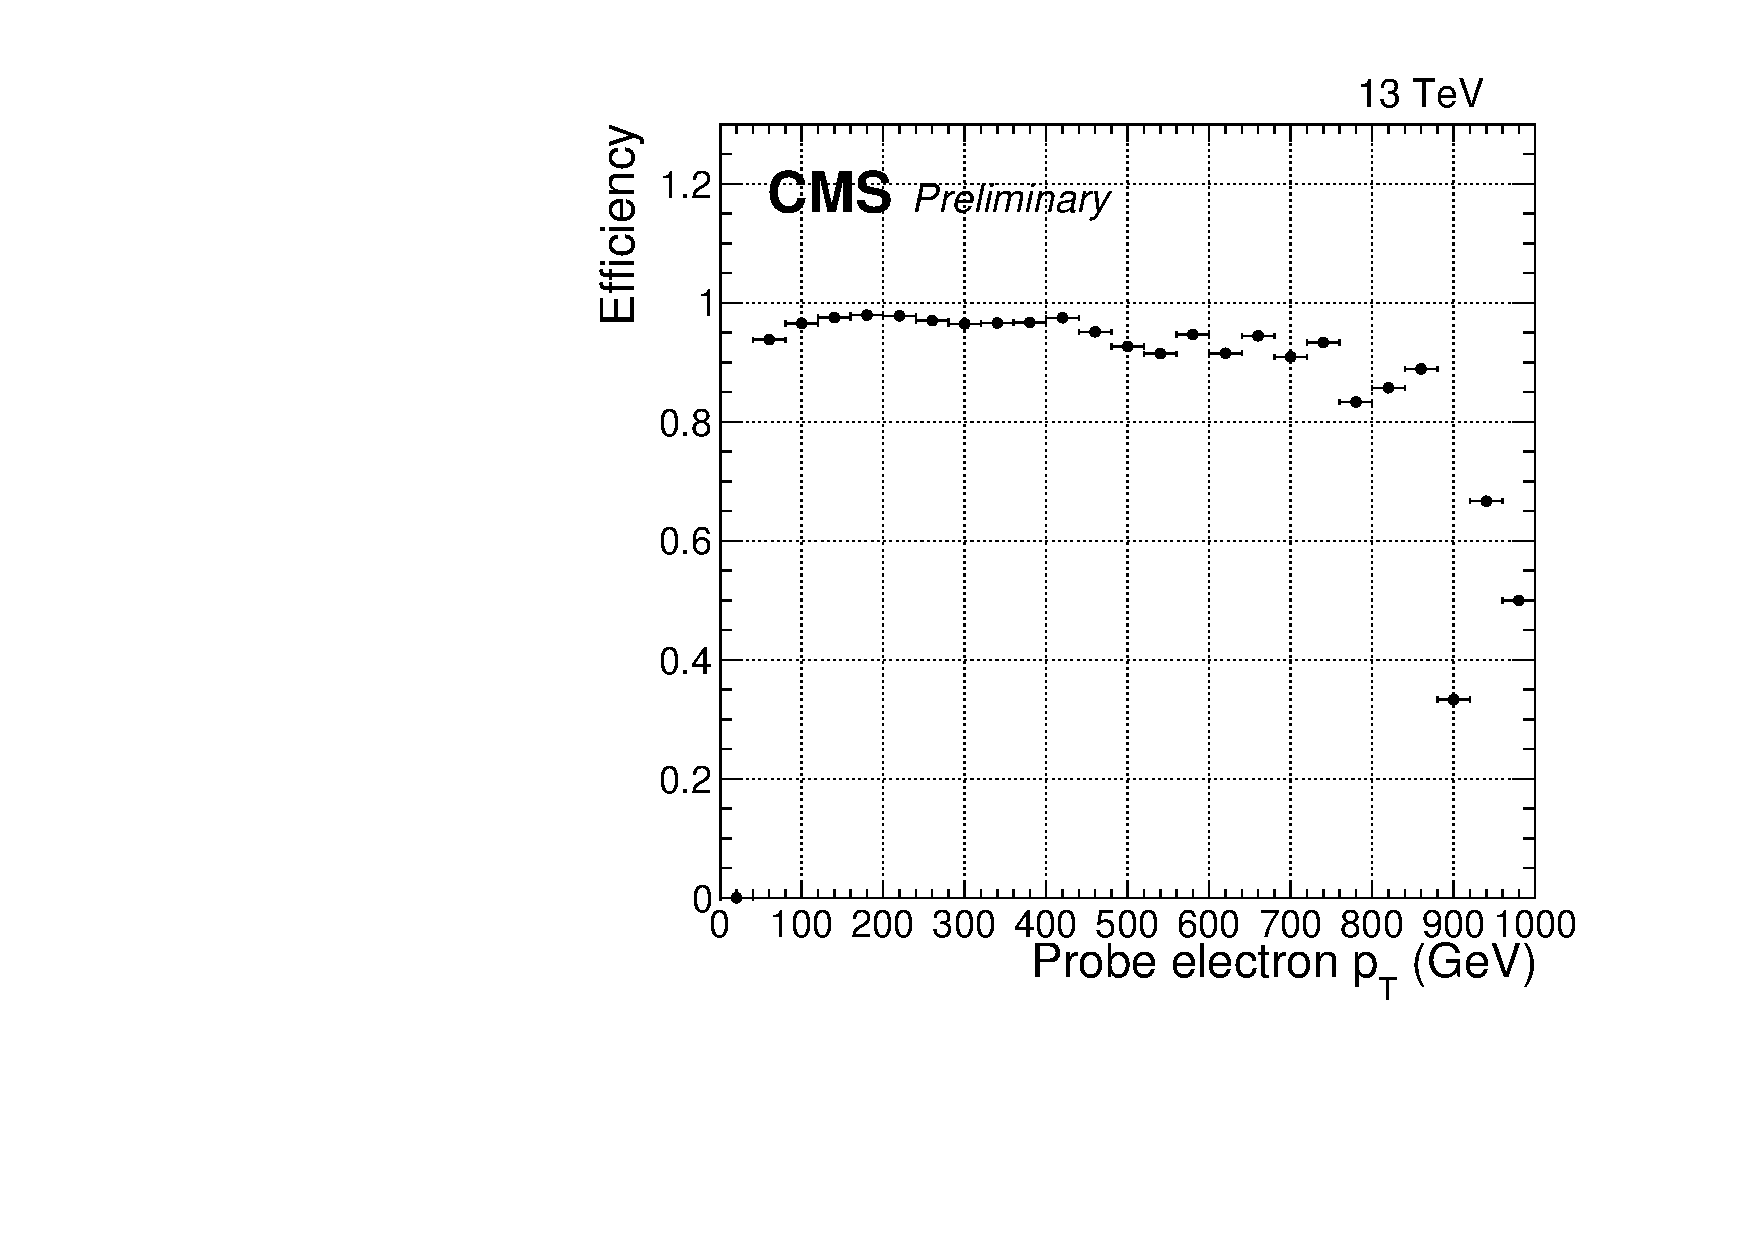
\includegraphics[width=0.475\textwidth]{figures/trigs/electron_barrel_trig.pdf}
%         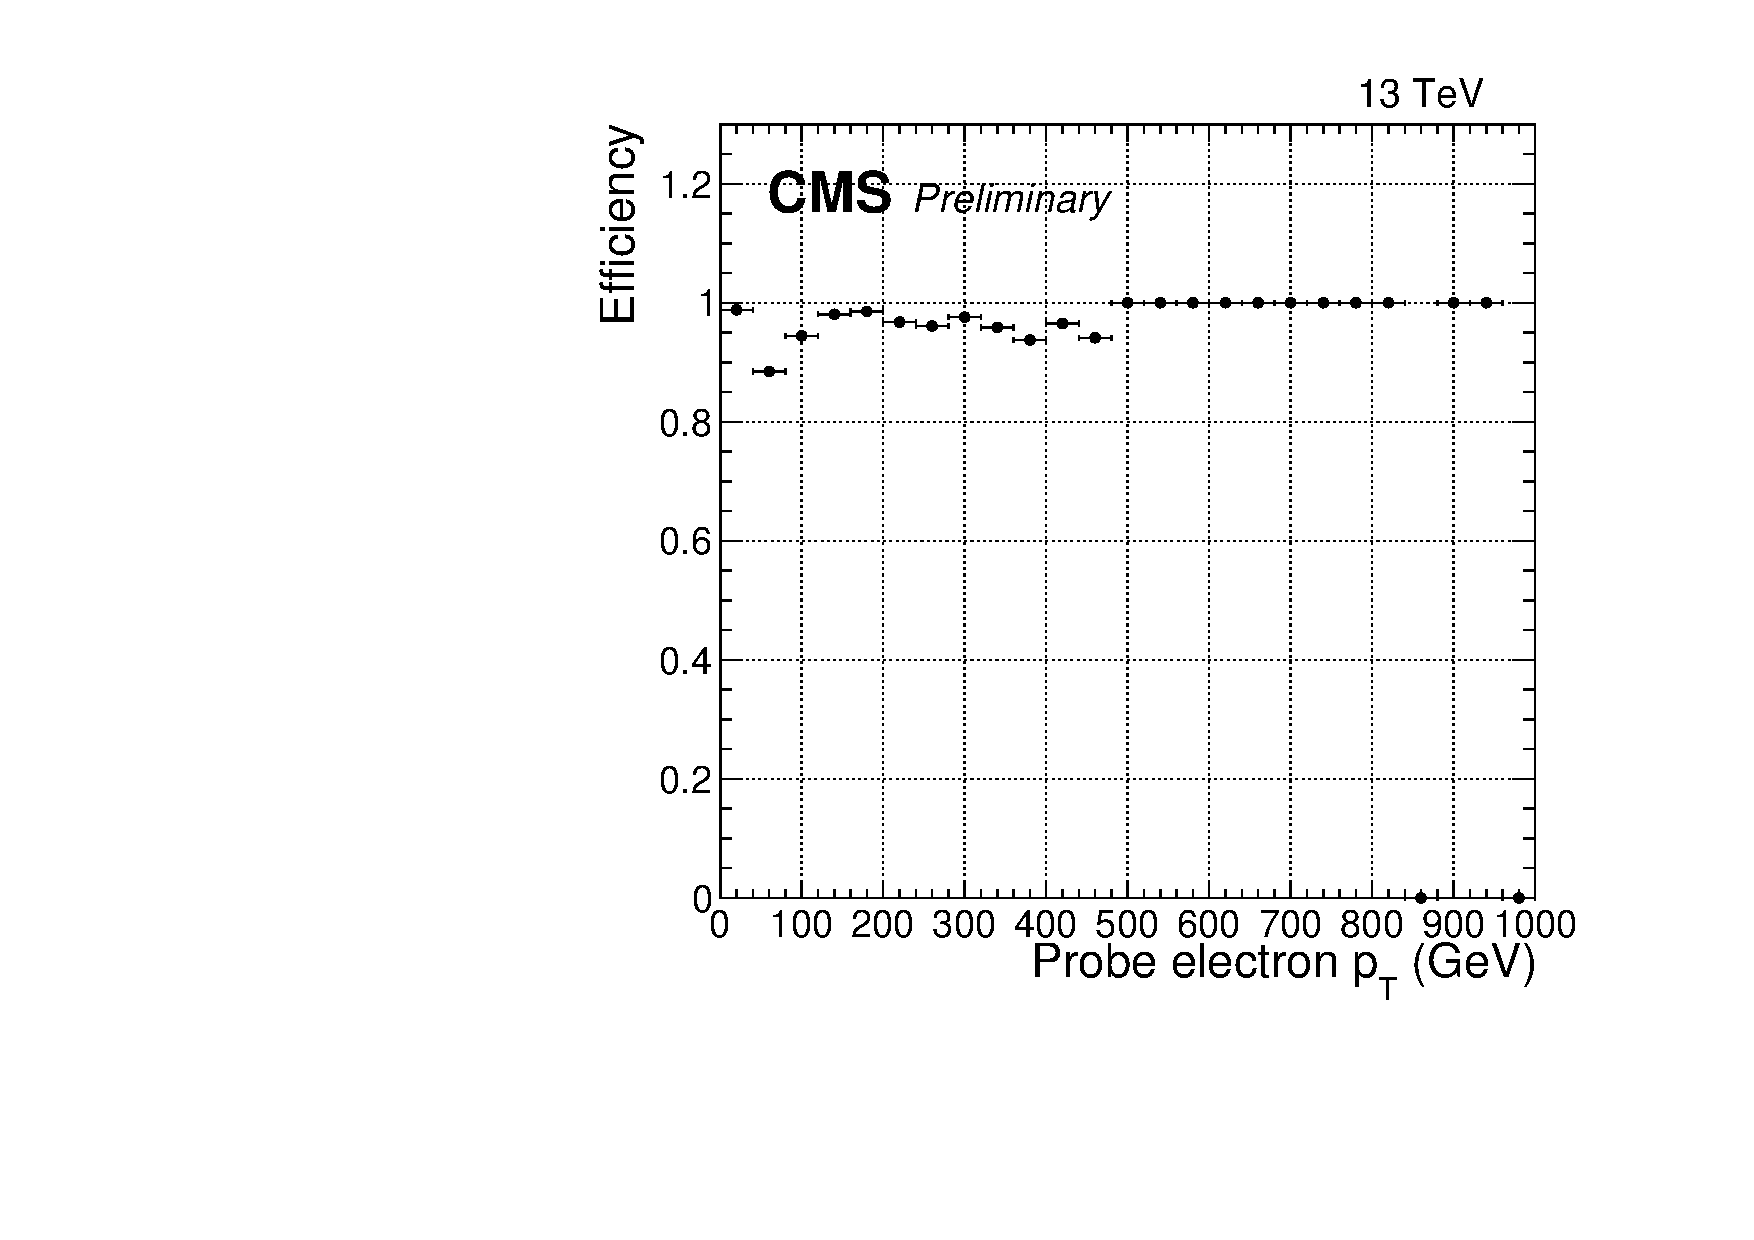
\includegraphics[width=0.475\textwidth]{figures/trigs/electron_endcap_trig.pdf}\\
%         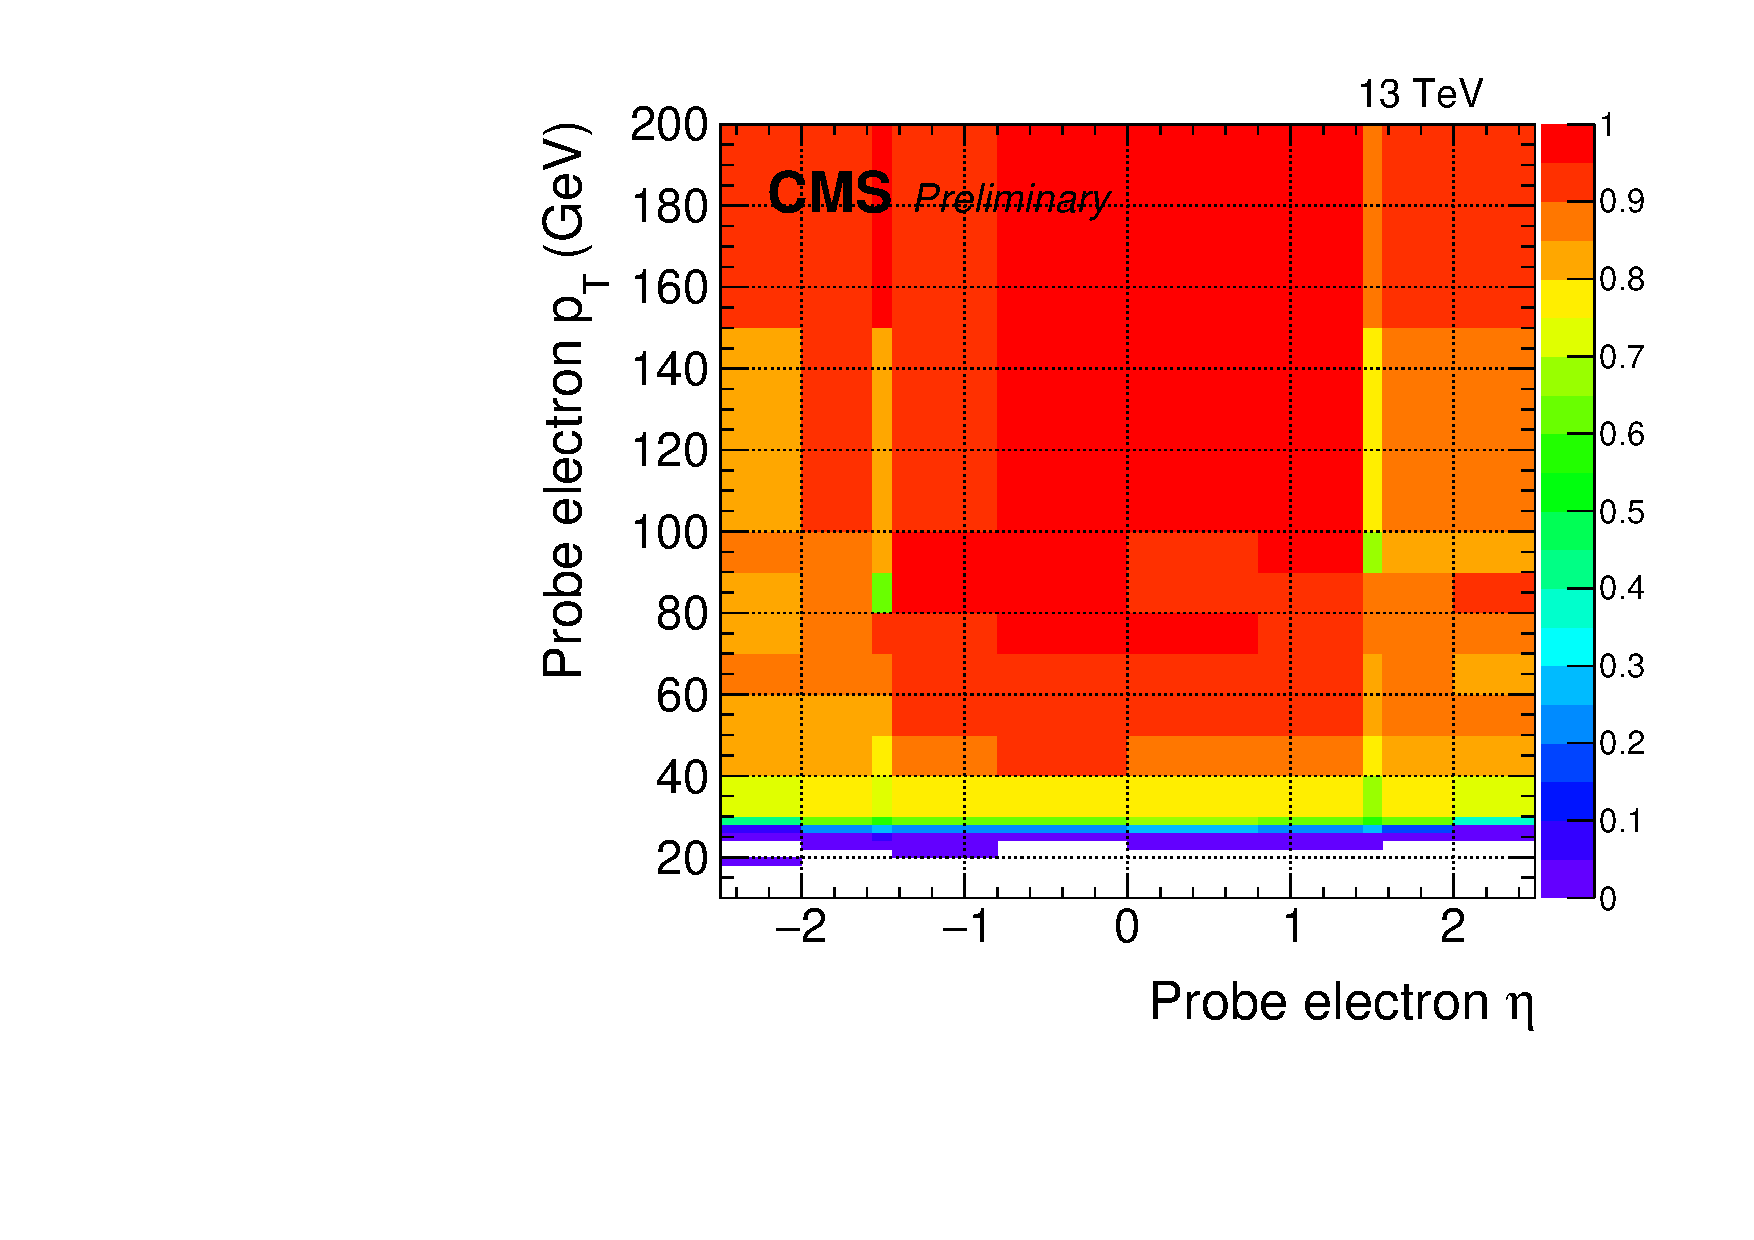
\includegraphics[width=0.475\textwidth]{figures/trigs/electron_lowpt_trig.pdf}\\
%   \caption{Efficiency of MET and METNoMu triggers as a function of offline \ETm~(upper left); efficiency of photon triggers (upper right); efficiency of single electron triggers for barrel/endcap (middle left/right); efficiency of single electron triggers at low $p_\text{T}$ ($<100$\,GeV). 
%   }
%   \label{fig:trigs}
% \end{figure}

\begin{figure}[hbtp]\begin{center}
    \subfloat[][]{
      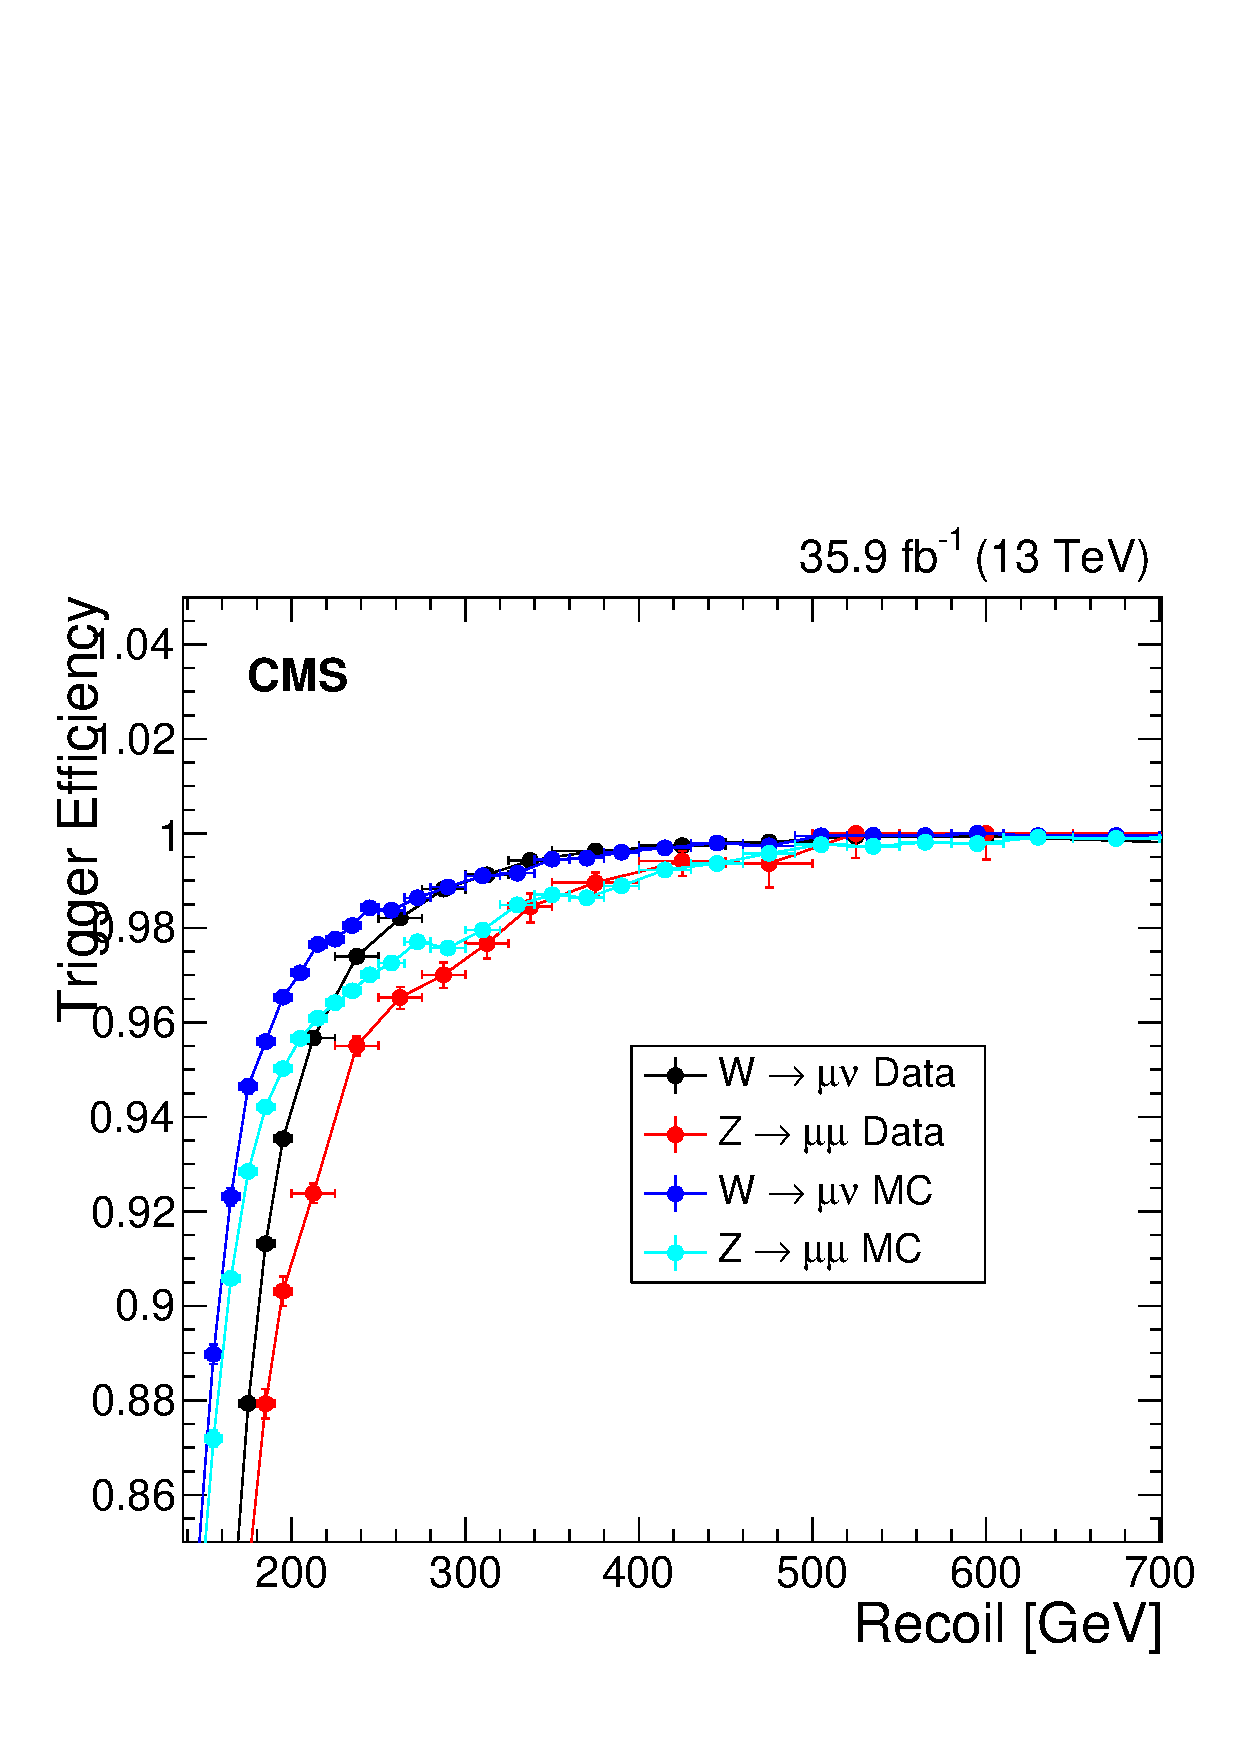
\includegraphics[width=0.45\textwidth]{figures/trigs/comparisonTurnOn_Wmn_Zmm_before_fix.pdf}
    }
    \subfloat[][]{
      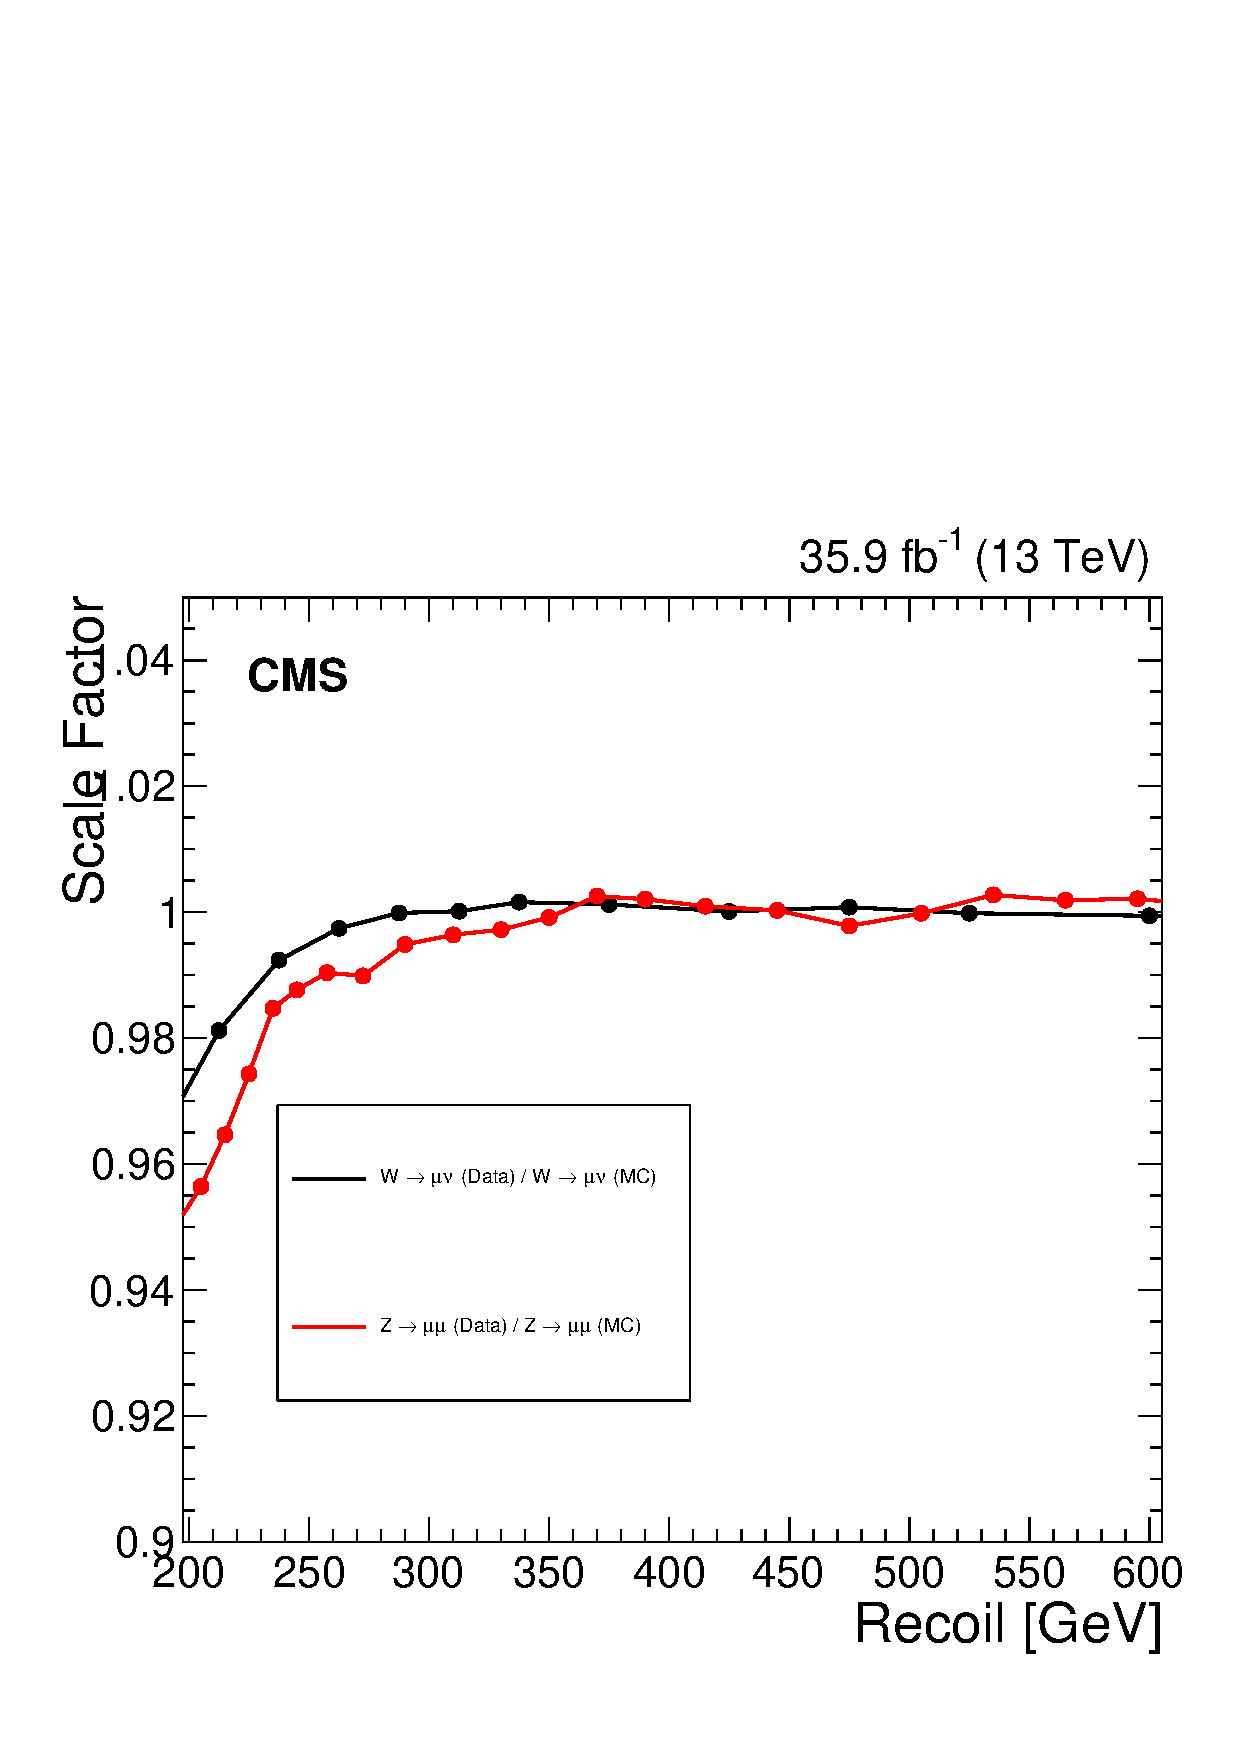
\includegraphics[width=0.45\textwidth]{figures/trigs/scale_factor_trigger_wmn_zmm_before_fix.pdf}
    }
    \caption{Comparison on both data and MC between the METNoMu+MHTNoMu trigger efficiency turn on as measured in \Wmn~and \Zmm~events (left). (Right) Comparison between the data to MC scale factors which show a significant disagreement in the low recoil region; taken from~\cite{CMS_AN_2016-473}.}
\label{fig:triggerComparison_wmn_zmm}\end{center}\end{figure}

\begin{figure}[hbtp]\begin{center}
      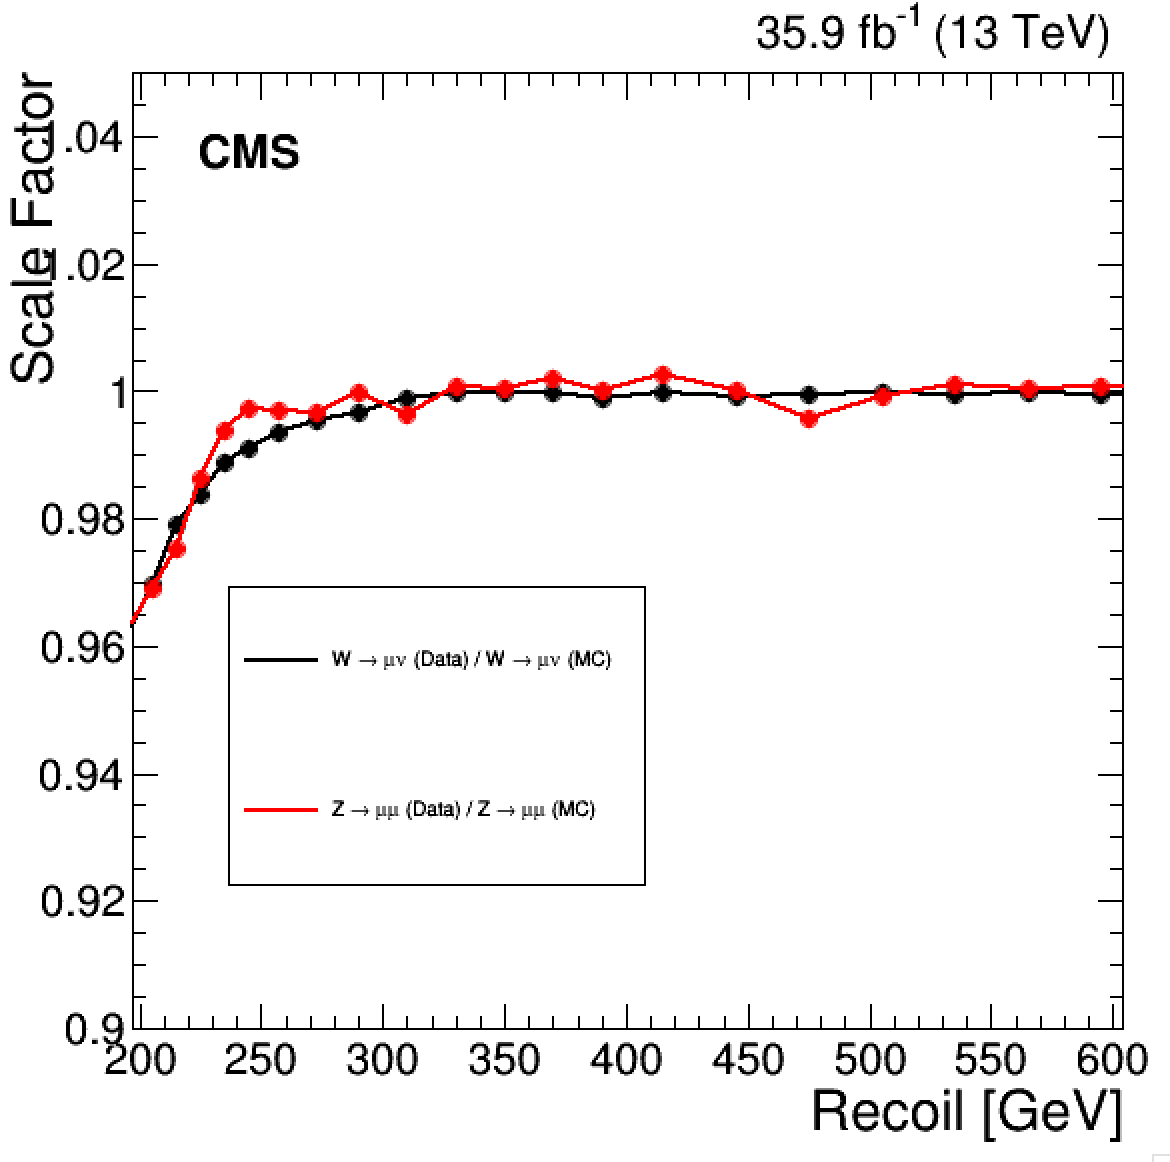
\includegraphics[width=0.45\textwidth]{figures/trigs/scale_factor_trigger_wmn_zmm_after_fix.png}
      \caption{
        Comparison between the data to MC scale factors as obtained computing the MET trigger turn-on in \Wmn~and \Zmm~events, which nicely agree over the full recoil spectrum after requiring to have a number of HLT muons equal to the number of the identified offline muons in the event; taken from~\cite{CMS_AN_2016-473}.}
      \label{fig:trigger_eff_corr}\end{center}\end{figure}

\begin{figure}[hbtp]\begin{center}
      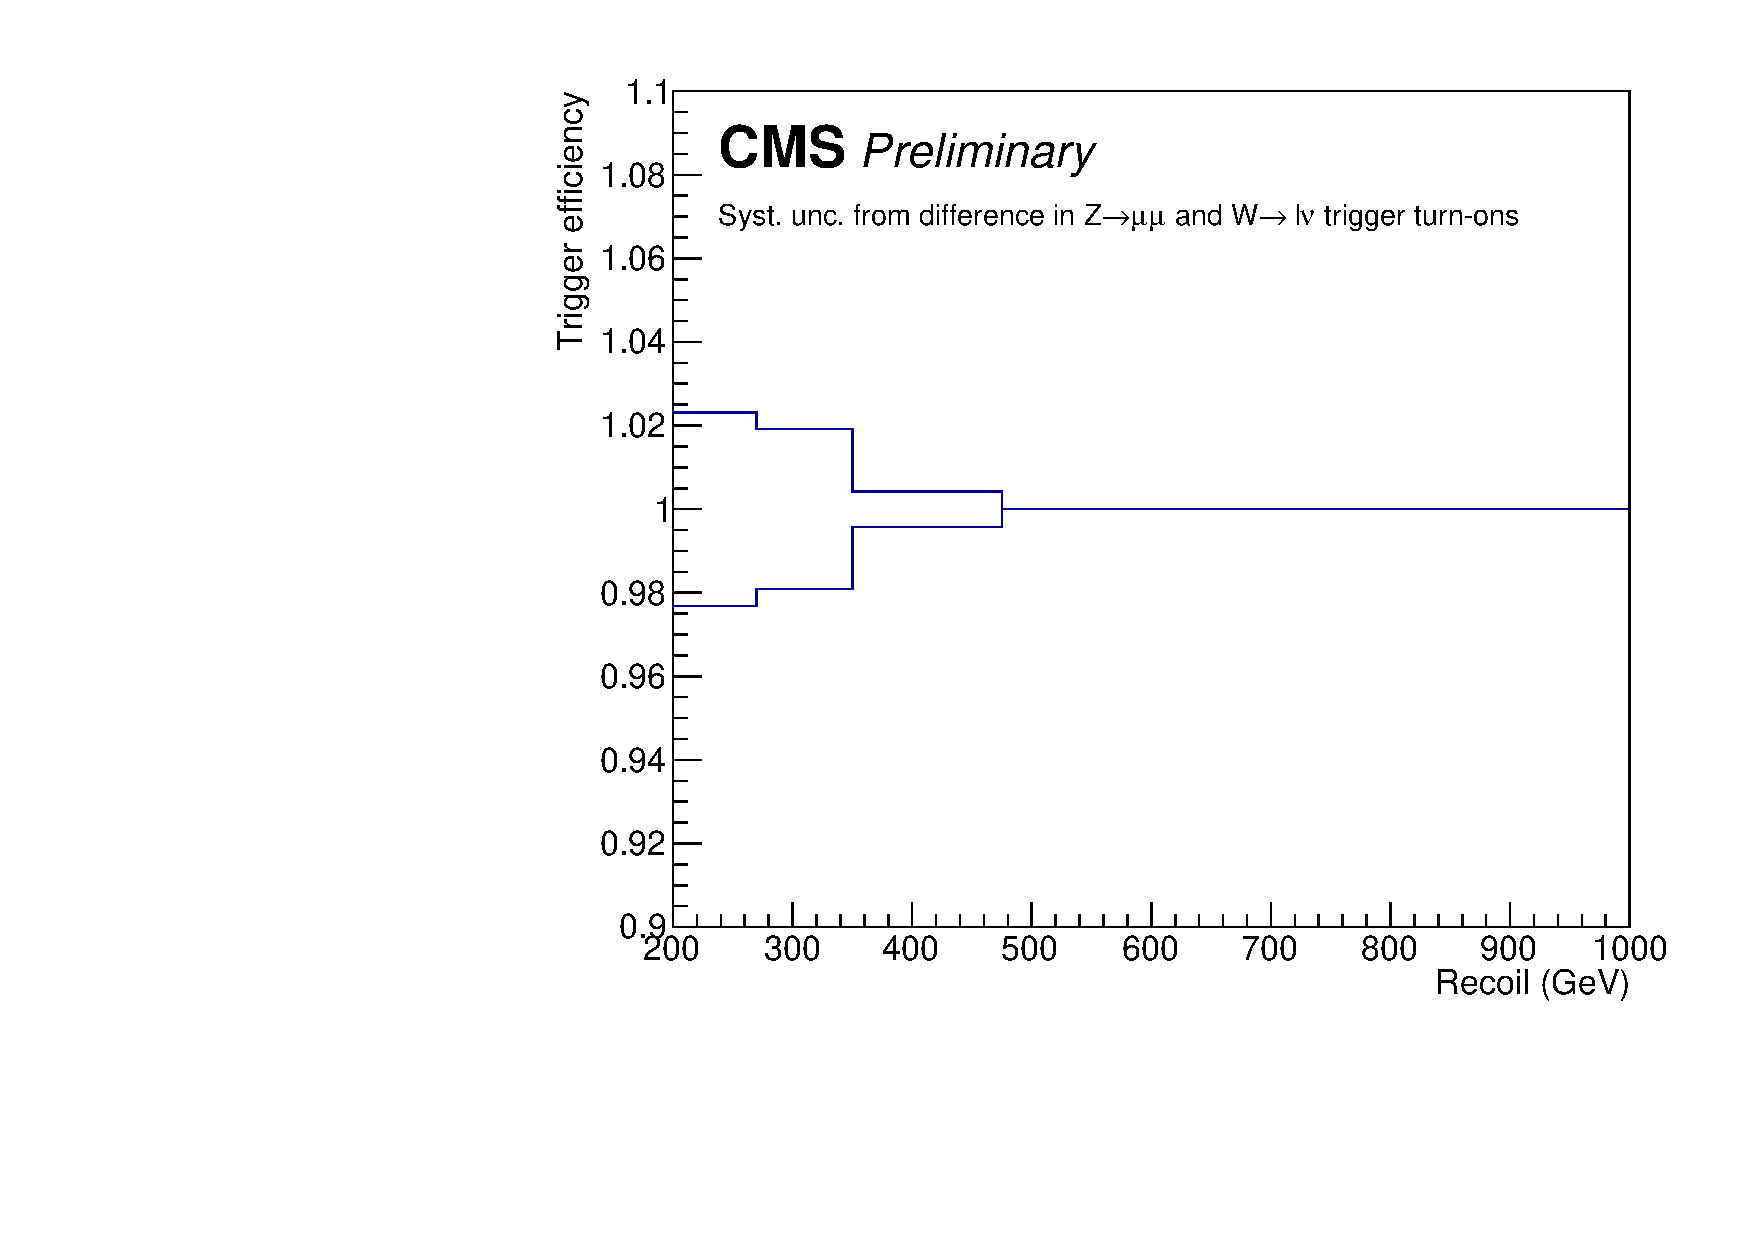
\includegraphics[width=0.45\textwidth]{figures/trigs/fixtrig_monoh.pdf}
      \caption{ Uncertainty on applied trigger weights in the \Zmm~control region due to the different METNoMu+MHTNoMu trigger efficiencies  in \Wmn~and \Zmm~events.
}
      \label{fig:fixtrig_monoh}\end{center}\end{figure}


\begin{figure}[hbtp]\begin{center}
    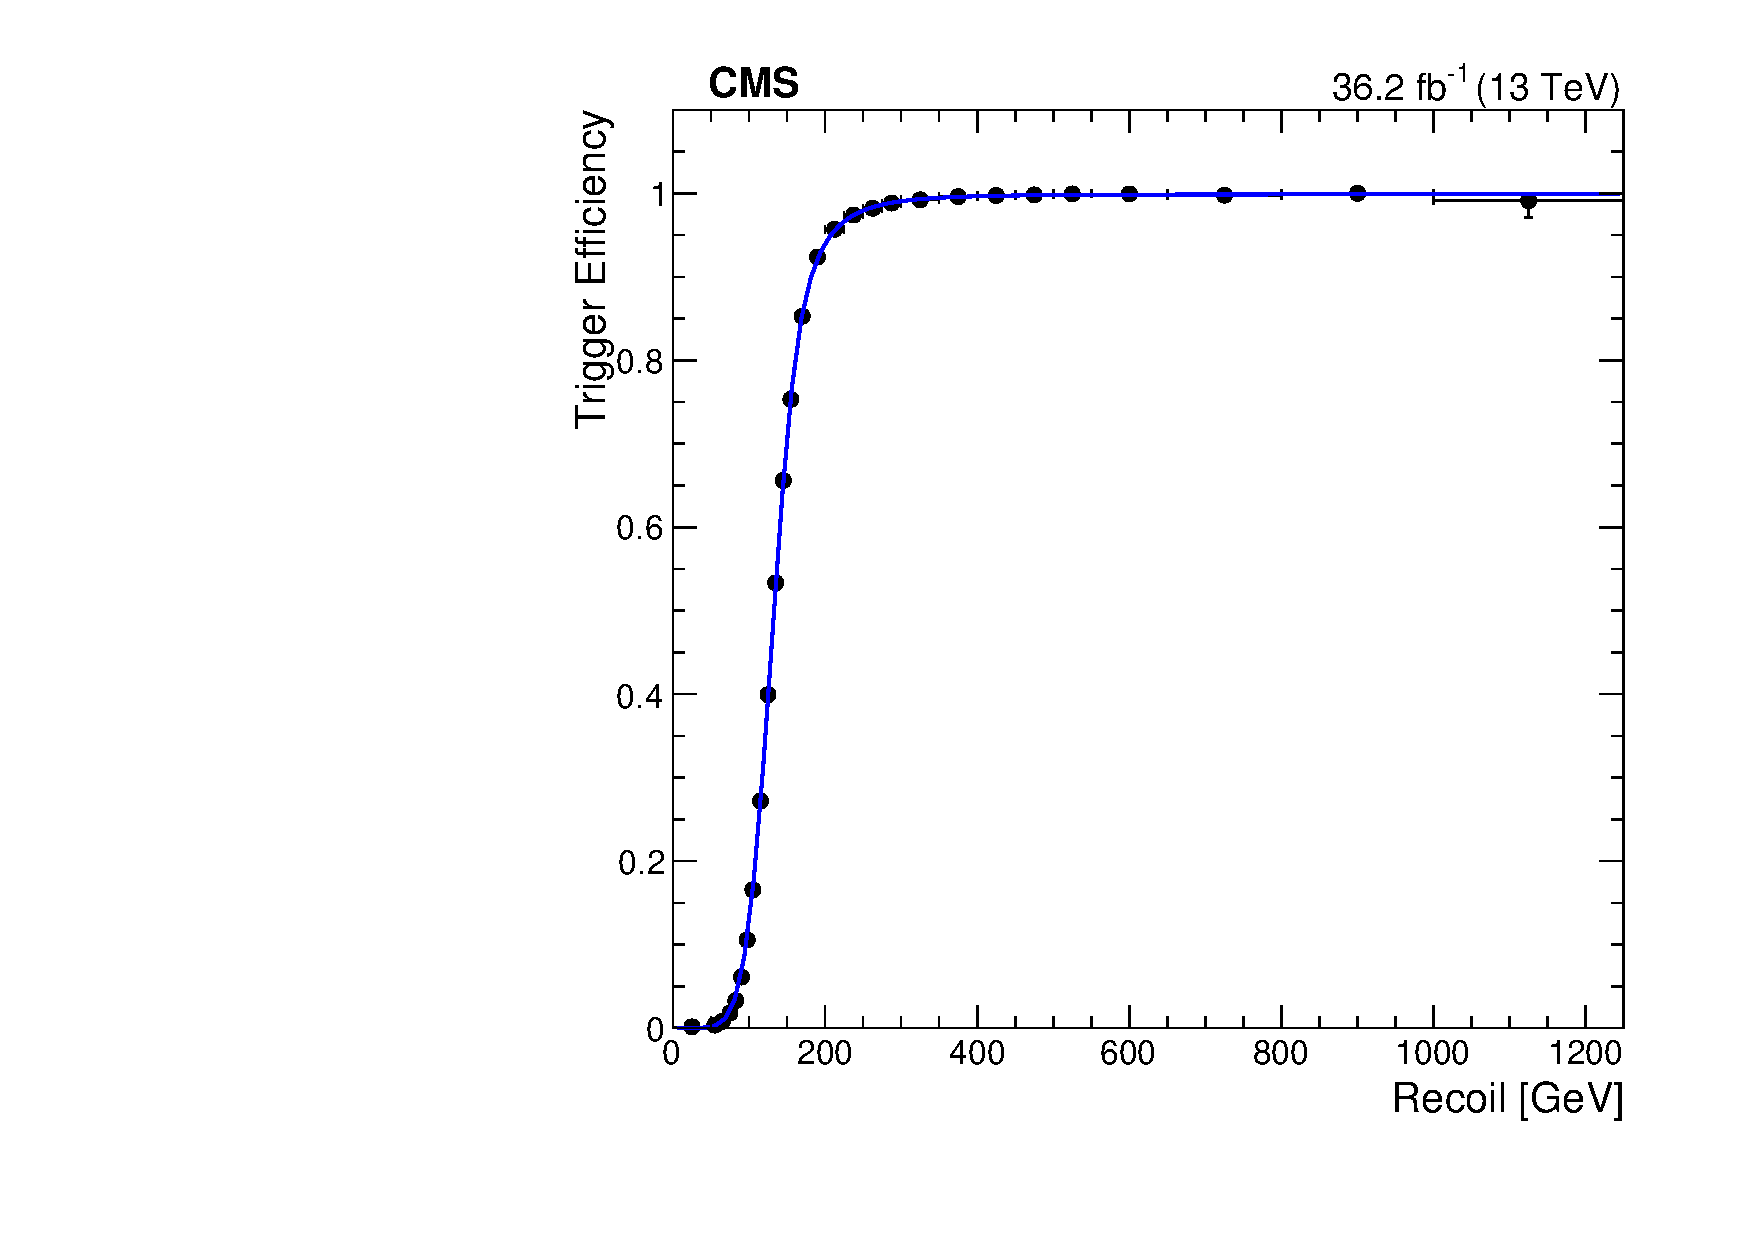
\includegraphics[height=0.45\textwidth,width=0.45\textwidth]{figures/trigs/metTriggerEff_mu.pdf}
    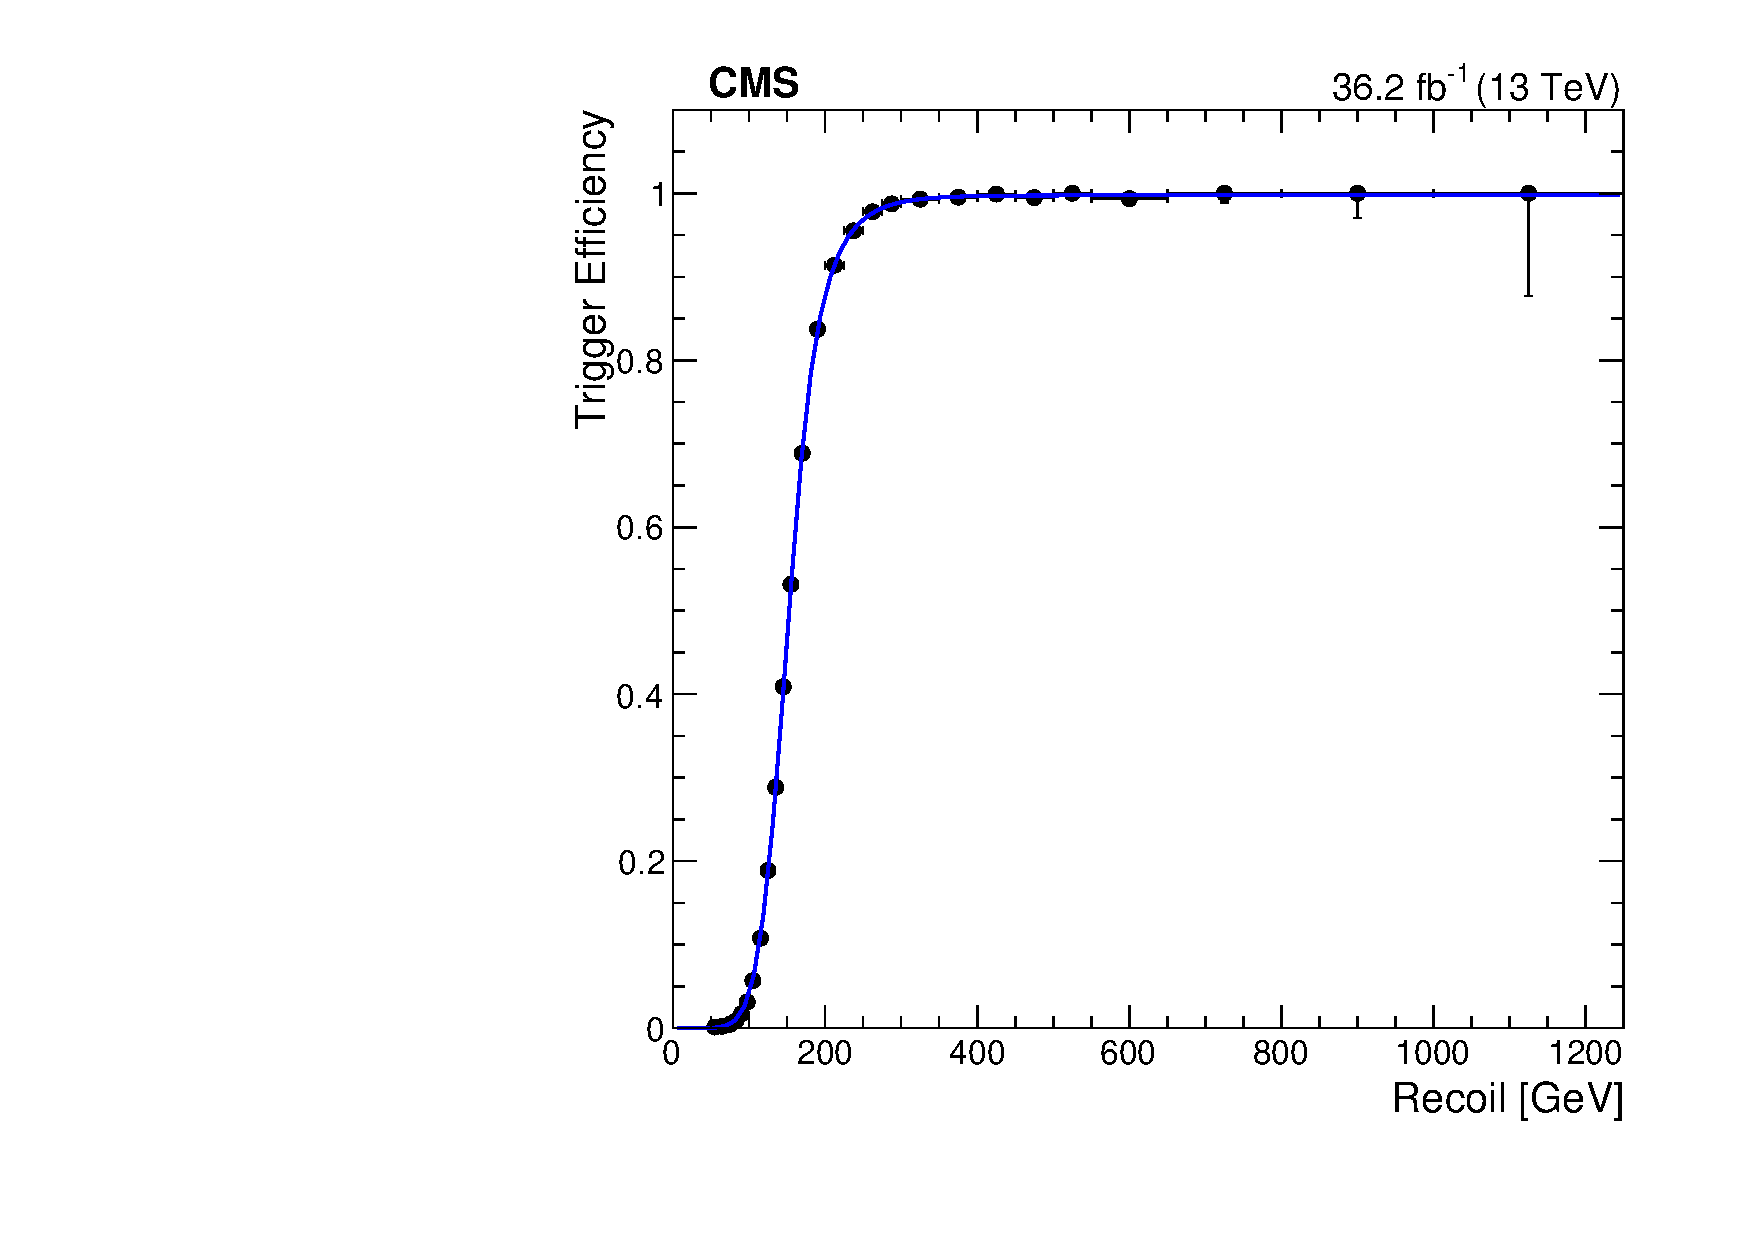
\includegraphics[height=0.45\textwidth,width=0.45\textwidth]{figures/trigs/metTriggerEff_el.pdf}
        \caption{MET trigger turn-on curve measured in single muon events (left) and single electron events (right). In the case of the single muon events, the trigger turn-on is computed as a function of the recoil (\MET without including the muon), while in the case of the single electron events it is computed as a function of \MET. Both measurements agree at the 1-2\% level at higher MET, and the efficiencies from the measurement in single muon events are applied to the simulated events in the analysis; taken from~\cite{CMS_AN_2016-473}. }
    \label{fig:hlteff_met}
 \end{center}\end{figure}


\begin{figure}[h!]
  \begin{center}
          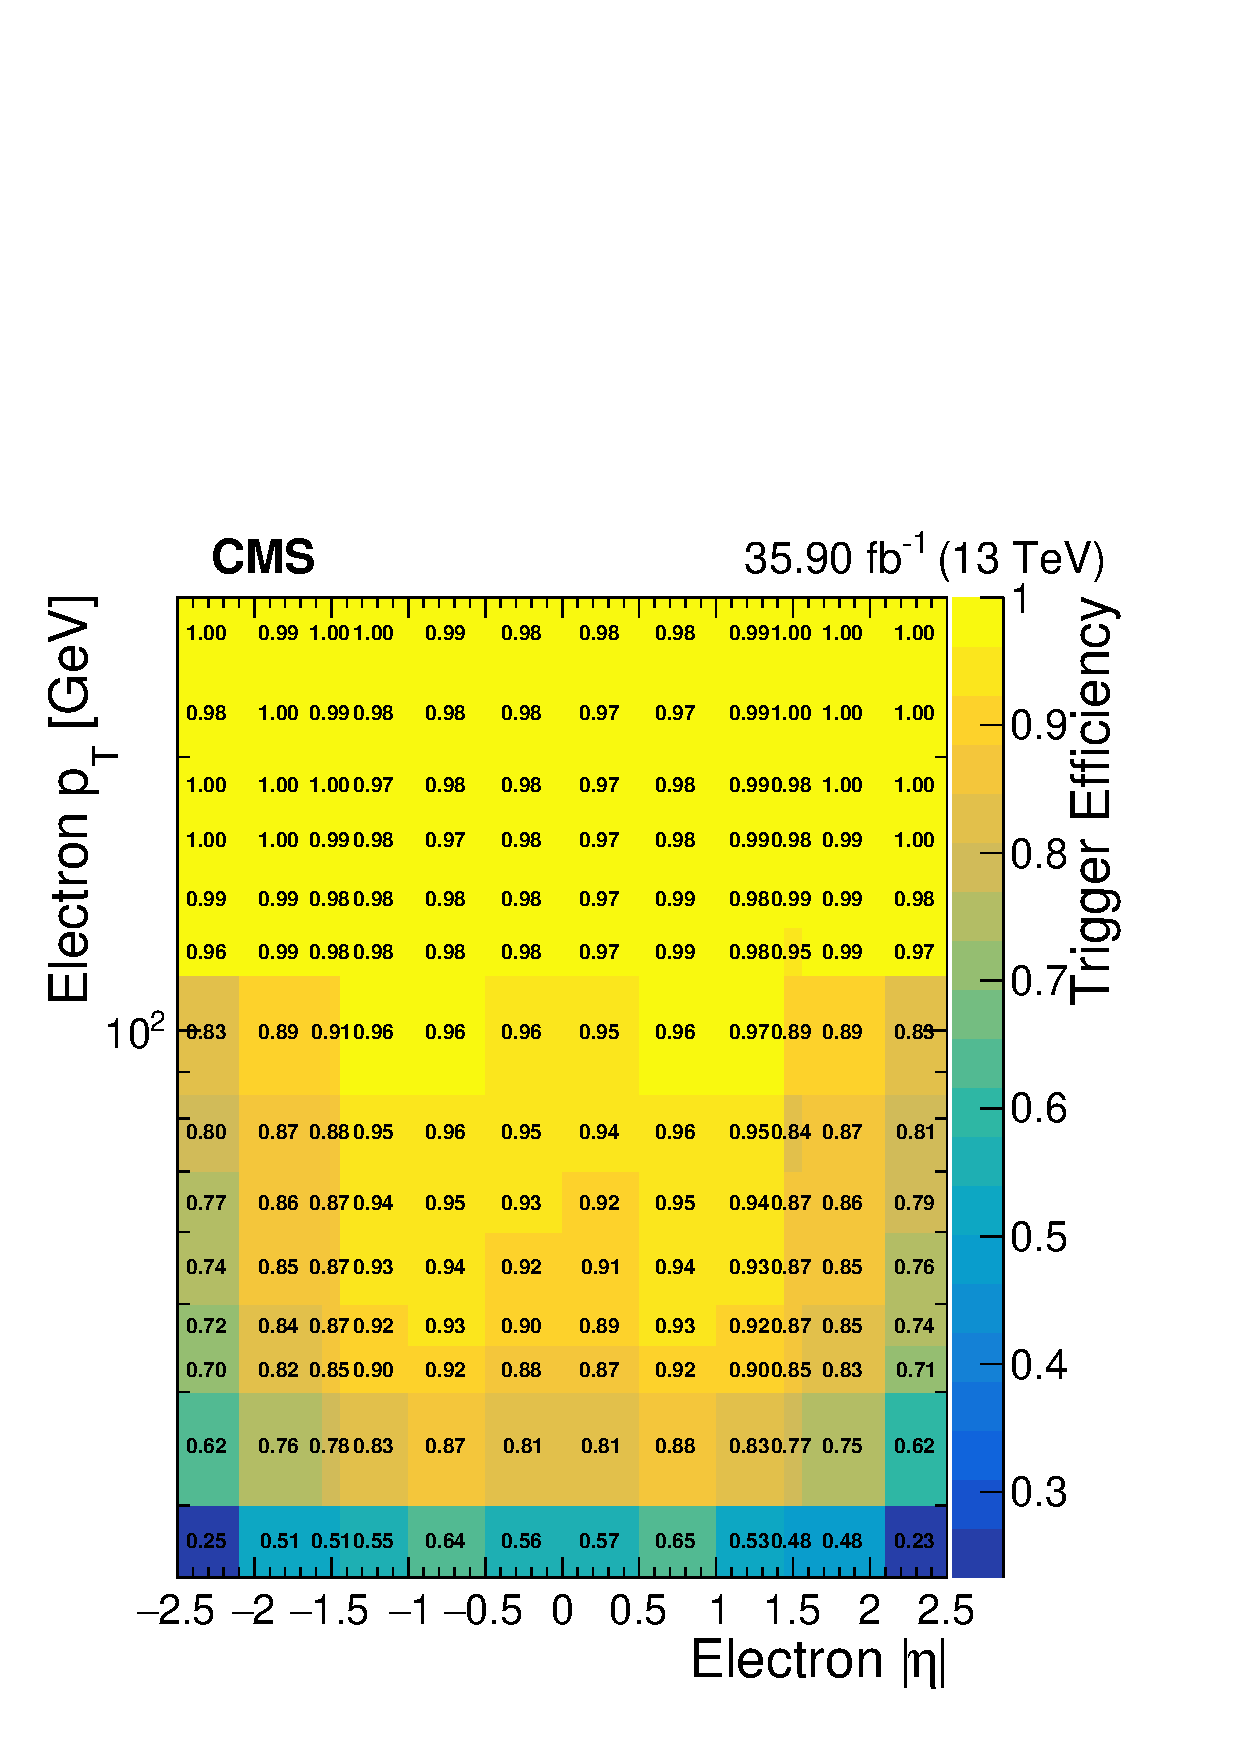
\includegraphics[width=0.40\textwidth]{figures/trigs/trgeff_ele_pt35.pdf}
          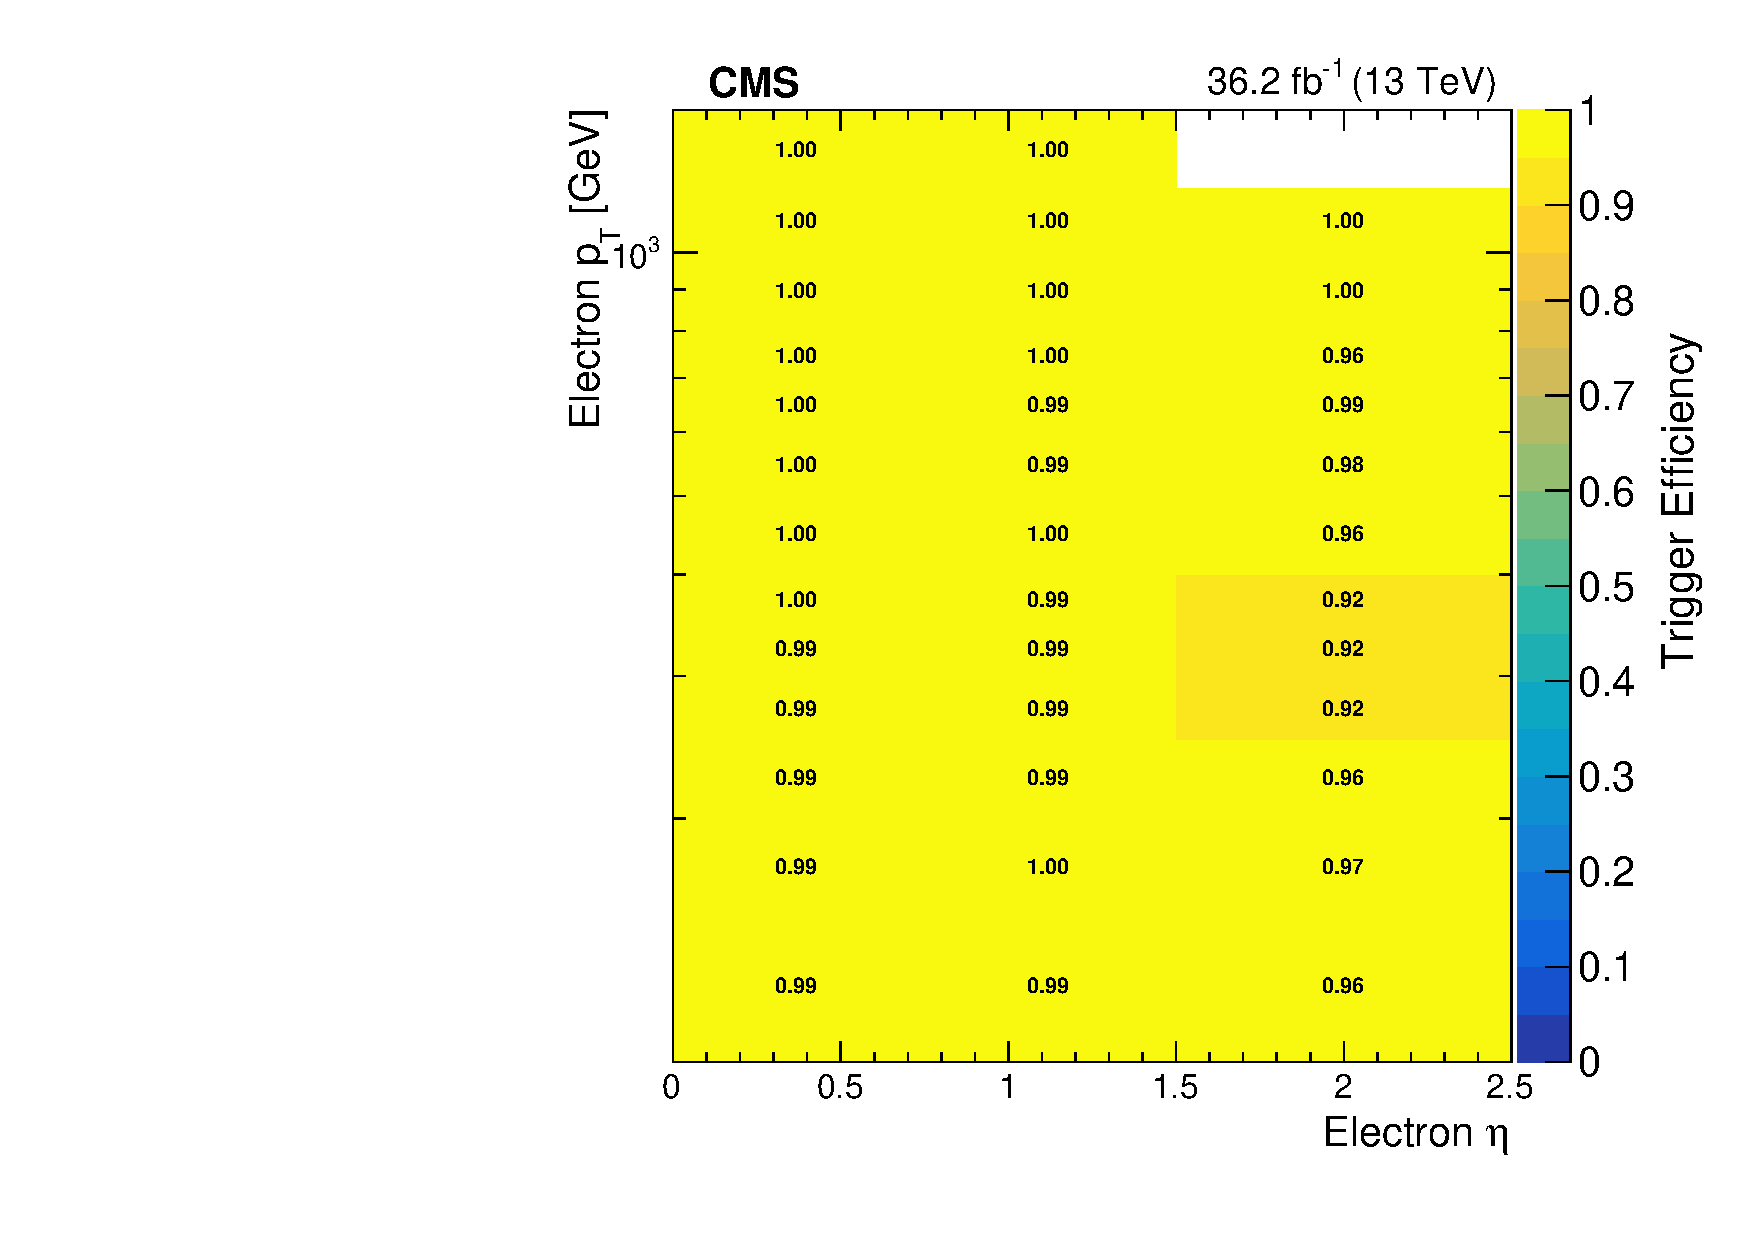
\includegraphics[width=0.42\textwidth]{figures/trigs/effetapt_jetht.pdf}
   \caption{Single electron trigger efficiencies as a function of electron \pt and $\eta$. The left plot shows the trigger efficiencies measured using Z tag-n-probe starting with electron \pt of 20 \GeV. The right one shows the electron trigger efficiency measured in the JetHT dataset using events passing the PFHT650 or PFHT800 trigger, starting at electron \pt of 100 \GeV; taken from~\cite{CMS_AN_2016-473}.}
   \label{fig:eltrigsfsplot}
  \end{center}
\end{figure}


\subsection{Background Monte Carlo Samples}

A list of all background MC samples and the corresponding cross-sections are given in Table~\ref{tab:bgmc}

{ \footnotesize

\centering
\begin{table}[htbp]\footnotesize
\begin{center}
  \caption{List of background MC samples. Datasets marked with * are LO in QCD and EWK but will have NLO corrections applied. Cross-sections marked with $\dag$ are (N)NLO} \label{tab:bgmc}
\begin{tabular}{|l|c|}
  \hline
  Dataset name & $\sigma$ [pb] \\
  \hline
/QCD\_HT200to300\_TuneCUETP8M1\_13TeV-madgraphMLM-pythia8 & $1735000$\\
/QCD\_HT300to500\_TuneCUETP8M1\_13TeV-madgraphMLM-pythia8 & $366800$\\
/QCD\_HT500to700\_TuneCUETP8M1\_13TeV-madgraphMLM-pythia8 & $29370$\\
/QCD\_HT700to1000\_TuneCUETP8M1\_13TeV-madgraphMLM-pythia8 & $6524$\\
/QCD\_HT1000to1500\_TuneCUETP8M1\_13TeV-madgraphMLM-pythia8 & $1064$\\
/QCD\_HT1500to2000\_TuneCUETP8M1\_13TeV-madgraphMLM-pythia8 & $121.5$\\
/QCD\_HT2000toInf\_TuneCUETP8M1\_13TeV-madgraphMLM-pythia8 & $25.42$\\
/ST\_t-channel\_top\_4f\_inclusiveDecays\_13TeV-powhegV2-madspin-pythia8\_TuneCUETP8M1 & $136.02^\dag$\\
/ST\_t-channel\_antitop\_4f\_inclusiveDecays\_13TeV-powhegV2-madspin-pythia8\_TuneCUETP8M1 & $80.95^\dag$\\
/ST\_tW\_antitop\_5f\_inclusiveDecays\_13TeV-powheg-pythia8\_TuneCUETP8M1 & $35.85^\dag$\\
/ST\_tW\_top\_5f\_inclusiveDecays\_13TeV-powheg-pythia8\_TuneCUETP8M1 & $35.85^\dag$\\
/ZH\_HToBB\_ZToNuNu\_M125\_13TeV\_powheg\_pythia8 & $0.08912$ \\
/ZH\_HToBB\_ZToLL\_M125\_13TeV\_powheg\_pythia8 & $0.04865$ \\
/ggZH\_HToBB\_ZToNuNu\_M125\_13TeV\_powheg\_pythia8 & $0.014366$ \\
/ggZH\_HToBB\_ZToLL\_M125\_13TeV\_powheg\_pythia8 & $0.007842$ \\
/WminusH\_HToBB\_WToLNu\_M125\_13TeV\_powheg\_pythia8 & $0.100$ \\
/WplusH\_HToBB\_WToLNu\_M125\_13TeV\_powheg\_pythia8 & $0.159$ \\
/ttHTobb\_M125\_13TeV\_powheg\_pythia8 & $0.506*0.5824$\\
/TT\_TuneCUETP8M2T4\_13TeV-powheg-pythia8 & $831.76^\dag$\\
/WW\_TuneCUETP8M1\_13TeV-pythia8 & $118.7^\dag$\\
/WZ\_TuneCUETP8M1\_13TeV-pythia8 & $47.2^\dag$\\
/ZZ\_TuneCUETP8M1\_13TeV-pythia8 & $16.6^\dag$\\
/DYJetsToLL\_M-50\_HT-100to200\_TuneCUETP8M1\_13TeV-madgraphMLM-pythia8* & $148.0$\\
/DYJetsToLL\_M-50\_HT-200to400\_TuneCUETP8M1\_13TeV-madgraphMLM-pythia8* & $40.94$\\
/DYJetsToLL\_M-50\_HT-400to600\_TuneCUETP8M1\_13TeV-madgraphMLM-pythia8* & $5.497$\\
/DYJetsToLL\_M-50\_HT-600to800\_TuneCUETP8M1\_13TeV-madgraphMLM-pythia8* & $1.367$\\
/DYJetsToLL\_M-50\_HT-800to1200\_TuneCUETP8M1\_13TeV-madgraphMLM-pythia8* & $0.6304$\\
/DYJetsToLL\_M-50\_HT-1200to2500\_TuneCUETP8M1\_13TeV-madgraphMLM-pythia8* & $0.1514$\\
/DYJetsToLL\_M-50\_HT-2500toInf\_TuneCUETP8M1\_13TeV-madgraphMLM-pythia8* & $0.003565$\\
/WJetsToLNu\_HT-100To200\_TuneCUETP8M1\_13TeV-madgraphMLM-pythia8* & $1343$\\
/WJetsToLNu\_HT-200To400\_TuneCUETP8M1\_13TeV-madgraphMLM-pythia8* & $359.6$\\
/WJetsToLNu\_HT-400To600\_TuneCUETP8M1\_13TeV-madgraphMLM-pythia8* & $48.85$\\
/WJetsToLNu\_HT-600To800\_TuneCUETP8M1\_13TeV-madgraphMLM-pythia8* & $12.05$ \\
/WJetsToLNu\_HT-800To1200\_TuneCUETP8M1\_13TeV-madgraphMLM-pythia8* & $5.501$ \\
/WJetsToLNu\_HT-1200To2500\_TuneCUETP8M1\_13TeV-madgraphMLM-pythia8* & $1.329$ \\
/WJetsToLNu\_HT-2500ToInf\_TuneCUETP8M1\_13TeV-madgraphMLM-pythia8* & $0.03216$ \\
/ZJetsToNuNu\_HT-100To200\_13TeV-madgraph* & $280.5$ \\
/ZJetsToNuNu\_HT-200To400\_13TeV-madgraph* & $77.7$\\
/ZJetsToNuNu\_HT-400To600\_13TeV-madgraph* & $10.71$\\
/ZJetsToNuNu\_HT-600To800\_13TeV-madgraph* & $2.559$\\ 
/ZJetsToNuNu\_HT-800To1200\_13TeV-madgraph* & $1.183$\\
/ZJetsToNuNu\_HT-1200To2500\_13TeV-madgraph* & $0.292$\\
/ZJetsToNuNu\_HT-2500ToInf\_13TeV-madgraph* & $0.0069$ \\
  \hline
  \end{tabular}
  \end{center}
\end{table}

}

NLO QCD and electroweak correction factors are applied to the W and Z
boson samples depending on the boson $\pt$. They are listed in
Tab.~\ref{tab:nlokfacw} and Tab.~\ref{tab:nlokfacz}.


\begin{table}[htbp]
\centering
  \caption{NLO $k$ factors for QCD and EW corrections for the W+jets simulation, depending on the \pt of the generated W boson.} \label{tab:nlokfacw}
  \begin{tabular}{cccc}
  \hline
  From W \pt & to W \pt & QCD $k$ factor & EW $k$ factor\\
  \hline
150 & 170 & 1.43896 & 0.966481 \\
170 & 200 & 1.45307 & 0.958351 \\
200 & 230 & 1.41551 & 0.948513 \\
230 & 260 & 1.42199 & 0.938304 \\
260 & 290 & 1.3477 & 0.929394 \\
290 & 320 & 1.35302 & 0.919688 \\
320 & 350 & 1.34289 & 0.910425 \\
350 & 390 & 1.32474 & 0.900288 \\
390 & 430 & 1.23267 & 0.889122 \\
430 & 470 & 1.22641 & 0.877255 \\
470 & 510 & 1.23149 & 0.86653 \\
510 & 550 & 1.21593 & 0.856032 \\
550 & 590 & 1.16506 & 0.84536 \\
590 & 640 & 1.01718 & 0.834675 \\
640 & 690 & 1.01575 & 0.822288 \\
690 & 740 & 1.05425 & 0.810779 \\
740 & 790 & 1.05992 & 0.799689 \\
790 & 840 & 1.01503 & 0.788566 \\
840 & 900 & 1.01761 & 0.777413 \\
900 & 960 & 0.947195 & 0.765405 \\
960 & 1020 & 0.932754 & 0.753711 \\
1020 & 1090 & 1.00849 & 0.742262 \\
1090 & 1160 & 0.94805 & 0.72925 \\
1160 & 1250 & 0.86956 & 0.716423 \\
  \hline
  \end{tabular}
\end{table}



\begin{table}[htbp]
\centering
  \caption{NLO $k$ factors for QCD and EW corrections for the Z+jets simulation, depending on the \pt of the generated Z boson.} \label{tab:nlokfacz}
  \begin{tabular}{cccc}
  \hline
  From Z \pt & to Z \pt & QCD $k$ factor & EW $k$ factor \\
  \hline
150 & 170 & 1.47528 & 0.970592 \\
170 & 200 & 1.5428 & 0.964424 \\
200 & 230 & 1.49376 & 0.956695 \\
230 & 260 & 1.39119 & 0.948747 \\
260 & 290 & 1.40538 & 0.941761 \\
290 & 320 & 1.44661 & 0.934246 \\
320 & 350 & 1.38176 & 0.927089 \\
350 & 390 & 1.37381 & 0.919181 \\
390 & 430 & 1.29145 & 0.909926 \\
430 & 470 & 1.33452 & 0.900911 \\
470 & 510 & 1.25765 & 0.892561 \\
510 & 550 & 1.24265 & 0.884353 \\
550 & 590 & 1.24331 & 0.8761 \\
590 & 640 & 1.16187 & 0.867687 \\
640 & 690 & 1.07349 & 0.858047 \\
690 & 740 & 1.10748 & 0.849014 \\
740 & 790 & 1.06617 & 0.840317 \\
790 & 840 & 1.05616 & 0.832017 \\
840 & 900 & 1.1149 & 0.823545 \\
900 & 960 & 1.03164 & 0.814596 \\
960 & 1020 & 1.06872 & 0.806229 \\
1020 & 1090 & 0.981645 & 0.798038 \\
1090 & 1160 & 0.81729 & 0.789694 \\
1160 & 1250 & 0.924246 & 0.781163 \\
  \hline
  \end{tabular}
\end{table}



